\documentclass[prl,aps,twocolumn,showpacs,superscriptaddress,longbibliography]{revtex4-1}

%altaffillsymbol
\usepackage{graphicx}% Include figure files
\usepackage{dcolumn}% Align table columns on decimal point
\usepackage{bm}% bold math
%\usepackage{dsfont}
\usepackage{amssymb,amsmath}
\usepackage{sidecap}
\usepackage{wrapfig}
%\usepackage[bookmarks]{hyperref}
\usepackage{natbib}
%\usepackage{braket}
\usepackage{dsfont}


%\bibliographystyle{apsrev}
%\nofiles
\usepackage{graphicx}
\usepackage{leftidx}
%\usepackage[caption=false]{subfig}
%\usepackage{caption}
%\usepackage{subcaption}
\usepackage{color}

\usepackage{bbold} %This package allows to write the identity symbol

\usepackage{wasysym} % In order to introduce polygon symbols in the text
%aus
%\usepackage[geometry]{ifsym}
%\usepackage{amsbsy}
%\usepackage{bbding}
%\usepackage{universal}
%\usepackage{showkeys}


\usepackage{stackrel}

% color for commenting
\newcommand{\col}[1]{\color{red} #1}
% package for strikethrough
\usepackage{soul,xcolor}
\setstcolor{red}



% ENVIRONMENTS
\newcommand{\be}{\begin{equation}}
\newcommand{\ee}{\end{equation}}
\newcommand{\ba}{\begin{align}}
\newcommand{\ea}{\end{align}}
\newcommand{\sysb}{\left\{\begin{array}}
\newcommand{\syse}{\end{array}\right.}
\newcommand{\baa}{\begin{array}}
\newcommand{\eaa}{\end{array}}
\newcommand{\bs}{\begin{split}}
\newcommand{\es}{\end{split}}

\newcommand{\matb}{\left(\begin{array}}
\newcommand{\mate}{\end{array}\right)}


%VERTICAL SPACES
\newcommand{\vsii}{\vspace{2 mm}}
\newcommand{\vsiii}{\vspace{3 mm}}
\newcommand{\vsiv}{\vspace{4 mm}}

% MEASURES
\newcommand{\ddk}{\int \frac{\rmd^{\left( d-1 \right)}k}{\left( 2\pi \right)^{\left( d-1 \right)}}}
\newcommand{\ddq}{\int \frac{d^{ d-1}q}{\left( 2\pi \right)^{\left( d-1 \right)}}}
\newcommand{\Dq}{\int \mathcal{D}q}
%\newcommand{\dd}[2]{\frac{\rmd^{#1}#2}{\left( 2\pi \right)^{#1 }}}
%\newcommand{\ddr}[2]{\frac{\rm{d}^{#1}#2}{\left( 2\pi \right)^{#1 }}}

% GENERIC SHORTHAND
\newcommand{\mal}{\mathcal}
\newcommand{\rmd}{{\rm{d}}}
\newcommand{\rmD}{{\rm{D}}}
\newcommand{\rme}[1]{{\rm{e}}^{#1}}
\newcommand{\mand}{\quad\text{ and }\quad}
\newcommand{\Dim}[1]{\left[ #1 \right]}
\newcommand{\vphi}{\varphi}
\newcommand{\wh}{\widehat}
\newcommand{\wt}{\widetilde}
\newcommand{\ob}{\mal{O}}
\newcommand{\id}{\mathbb{1}}
\newcommand{\trace}[1]{{\rm tr}\left\{ #1 \right\}}
\newcommand{\order}[1]{O\left( #1 \right)}
\newcommand{\ve}{\varepsilon}
\newcommand{\gh}{\phantom}
\newcommand{\EGamma}[1]{\Gamma \lt #1 \rt}
\newcommand{\ha}{\frac{1}{2}}
\newcommand{\eq}{\, = \,}



% SHORTHANDS SPECIFIC TO THE PRESENT TEXT
\newcommand{\pop}[1]{\hat{n}_{#1}}
\newcommand{\bp}{\mathbf{p}}
\newcommand{\bx}{\mathbf{x}}
\newcommand{\brho}{\bm{\rho}}
\newcommand{\brhoo}{\bm{\rho_0}}
\newcommand{\hsi}{\wh{\sigma}}
\newcommand{\whN}{\wh{N}}
\newcommand{\quadblock}[4]{\matb{c|c} #1 & #2 \\ \hline #3 & #4 \mate}
\newcommand{\bE}{{\bf E}}
\newcommand{\bD}{{\bf D}}
\newcommand{\ce}{\rho}
\newcommand{\sdim}[1]{\lqq #1 \rqq}
\newcommand{\tphi}{\widetilde{\vphi}}
\newcommand{\xp}{x_\perp}
\newcommand{\vth}{\vartheta}
\newcommand{\rmn}{{\rm n}}
\newcommand{\rmr}{{\rm r}}
\newcommand{\hatt}{\hat{t}}
\newcommand{\pp}{{\mathbf{P}}}
\newcommand{\tx}{\tilde{x}}
\newcommand{\ty}{\tilde{y}}



% BRACKETS
\newcommand{\lt}{\left(}
\newcommand{\rt}{\right)}
\newcommand{\lqq}{\left[}
\newcommand{\rqq}{\right]}
\newcommand{\lan}{\left\langle}
\newcommand{\ran}{\right\rangle}
\newcommand{\abs}[1]{\left| #1 \right|}
\newcommand{\eval}[1]{\left.\right|_{ #1 }}
\newcommand{\av}[1]{\lan #1 \ran}
\newcommand{\norm}[1]{\left\| #1 \right\|}
\newcommand{\set}[1]{\left\{  #1  \right\}}



% PAULI MATRICES (SIMBOLS AND MATRIX FORMS)
\newcommand{\sx}{{\sigma^x}}
\newcommand{\sy}{{\sigma^y}}
\newcommand{\sz}{{\sigma^z}}
\newcommand{\sxM}{\matb{cc} 0 & 1 \\ 1 & 0   \mate}
\newcommand{\syM}{\matb{cc} 0 & -i \\ i & 0   \mate}
\newcommand{\szM}{\matb{cc} 1 & 0 \\ 0 & -1   \mate}	
\newcommand{\stx}[1]{\widetilde{\sigma}_{#1}^x}
\newcommand{\sty}[1]{\widetilde{\sigma}_{#1}^y}
\newcommand{\stz}[1]{{\widetilde{\sigma}_{#1}^z}}

% NUMBER SETS
\newcommand{\R}{\mathbb{R}}
\newcommand{\N}{\mathbb{N}}
\newcommand{\Z}{\mathbb{Z}}
\newcommand{\C}{\mathbb{C}}

% QUANTUM MECHANICS
\newcommand{\ket}[1]{\left| #1 \ran}
\newcommand{\bra}[1]{\lan #1 \right|}
\newcommand{\bracket}[2]{\lan #1 \right| \!\left. #2 \ran}
\newcommand{\proj}[1]{\ket{#1} \bra{#1}}
\newcommand{\comm}[2]{\left[ #1, #2 \right]}
\newcommand{\acomm}[2]{\left\{ #1, #2 \right\}}




% TRIGONOMETRIC AND HYPERBOLIC FUNCTIONS
\newcommand{\cosa}[1]{\cos \left(  #1 \right)}
\newcommand{\sina}[1]{\sin \left(  #1 \right)}
\newcommand{\tana}[1]{\tan \left(  #1 \right)}
\newcommand{\cossa}[2]{\cos^{#1} \left(  #2 \right)}
\newcommand{\sinna}[2]{\sin^{#1} \left(  #2 \right)}
\newcommand{\tanna}[2]{\tan^{#1} \left(  #2 \right)}
\newcommand{\tann}[1]{\tan^{#1}}
\newcommand{\cosha}[1]{\cosh \left(  #1 \right)}
\newcommand{\sinha}[1]{\sinh \left(  #1 \right)}
\newcommand{\tanha}[1]{\tanh \left(  #1 \right)}
\newcommand{\cossha}[2]{\cosh^{#1} \left(  #2 \right)}
\newcommand{\sinnha}[2]{\sinh^{#1} \left(  #2 \right)}

% OTHER FUNCTIONS
\newcommand{\loga}[1]{\log \lt #1 \rt}
\newcommand{\lna}[1]{\ln \lt #1 \rt}
\newcommand{\BK}[2]{K_{#1} \lt #2 \rt}
\newcommand{\Prob}{\mathbb{P}}


\newcommand{\nol}{\nonumber \\}


\newcommand{\reff}[1]{(\ref{#1})}
\newcommand{\note}[1]{{\bf \small #1}}

% BOUNDS
\newcommand{\maxx}[2]{\max\limits_{#1}^{} \left\{ #2 \right\}}
\newcommand{\minn}[2]{\min\limits_{#1}^{} \left\{ #2 \right\}}

% LIMITS IN SUMS, INTEGRALS, AND THE LIKE
\newcommand{\prodl}[2]{\prod\limits_{#1}^{#2}}
\newcommand{\suml}[2]{\sum\limits_{#1}^{#2}}
\newcommand{\intl}[2]{\int_{#1}^{#2}}
\newcommand{\bol}[2]{\bigotimes\limits_{#1}^{#2}}
\newcommand{\liml}[1]{\lim\limits_{#1}}



% CORRECTIONS
\newcommand{\change}[1]{\textcolor{blue}{#1}}
\newcommand{\changer}[1]{\textcolor{red}{#1}}
\newcommand{\changeg}[1]{\textcolor{green}{#1}}
\newcommand{\changeb}[1]{\textcolor{blue}{#1}}
\newcommand{\tochange}[1]{\textcolor{magenta}{#1}}
\newcommand{\nochange}[1]{\textcolor{black}{#1}}
\newcommand{\mm}[1]{{\tochange{\footnotesize{\bf (#1)}}}}
\newcommand{\ag}[1]{{\footnotesize \changer{#1}}}
\newcommand{\jm}[1]{{\footnotesize \changeg{#1}}}
\newcommand{\comma}{\quad , \quad}

\newcommand{\dar}{\downarrow}
\newcommand{\uar}{\uparrow}


\newcommand{\transp}{\mathtt{T}}


\newcommand{\ind}{b}
\newcommand{\indd}{c}


\usepackage{amsthm}
\newtheorem{mydef}{Definition}
\newtheorem{prop}{Proposition}
\newtheorem{theorem}{Theorem}


 \newcommand{\up}{\uparrow}
 \newcommand{\uu}{\up\, \up}
 \newcommand{\down}{\downarrow}
 \newcommand{\dd}{\downarrow\, \downarrow}

  \newcommand{\tspace}{\rule{0pt}{2.6ex}}
  \newcommand{\norml}{\textnormal}
  \newcommand{\op}[1]{\mathrm{\hat{#1}}}

\begin{document}

\title{Synthetic lattices, flat bands and localization in Rydberg quantum simulators in the presence of disorder}

\author{Maike Ostmann}
\author{Matteo Marcuzzi}
\author{Ji\v{r}\'{i} Min\'{a}\v{r}}
\author{Igor Lesanovsky}
\affiliation{School of Physics and Astronomy, University of Nottingham, Nottingham, NG7 2RD, UK}
\affiliation{Centre for the Mathematics and Theoretical Physics of Quantum Non-equilibrium Systems,
University of Nottingham, Nottingham NG7 2RD, UK}



\begin{abstract}
The most recent manifestation of cold Rydberg atom quantum simulators that employs tailored optical tweezer arrays enables the study of many-body dynamics under so-called facilitation conditions. \changer{We show how the facilitation mechanism yields a Hilbert space structure in which the many-body states organize into synthetic lattices}, which feature in general one or several flat bands and may support immobile localized states. We focus our discussion on the simple case of a Rydberg ladder for which we analyze in particular the influence of disorder generated by the uncertainty of the atoms positions. The localization properties of this system are characterized through two localization lengths. Moreover, we discuss the experimental preparation of an immobile localized state, and analyze disorder-induced propagation effects which may be investigated experimentally.
\end{abstract}
\pacs{}
\maketitle


Over the past few decades, advances in the manipulation of cold and ultra-cold atomic gases rendered them into a versatile quantum simulation platform \cite{Bloch_2008,Bloch_2012}. Indeed, several paradigmatic many-body models have been studied experimentally, including the Luttinger liquid \cite{hofferberth2007}, Tonks-Girardeau gas \cite{kinoshita2004}, Bose-Hubbard \cite{greiner2002, greiner2003}, and Fermi-Hubbard \cite{Kohl2005}, permitting to directly observe several predicted phenomena, such as quantum revivals \cite{greiner2002_revival}, Lieb-Robinson bounds \cite{cheneau2012}, and topological phase transitions \cite{hadzibabic2006}.

Among many different physical systems apt to act as quantum simulators, ensembles of Rydberg atoms \cite{a_Saffman_RMP_10, Low_2012, Gallagher_1994} stand out for their strong interactions, which are now known to give rise to an intricate phenomenology, \changer{including devil's staircases \cite{Weimer2010, Levi2016, Lan2015}, aggregate formation and melting \cite{Schempp2014, Lan2016}, Rydberg crystals \cite{Schauss_2015}, optical bistability \cite{Carr2013, Sibalic2016} and phase transitions and universal scaling \cite{Low2009, Marcuzzi2014, Gutierrez2015}} \mm{In this form, however, we need many more works, which would end up flooding the introduction with references.}. These systems are currently employed for a variety of tasks, such as quantum information processing \cite{Jaksch2000,Weimer_2010,Saffman_2016} and the simulation of quantum spin systems \cite{Labuhn_2015, Schauss_2015}. Several among these instances employ the so-called \emph{anti-blockade} (or \emph{facilitation}) mechanism (see e.g., Refs.~\cite{Ates_2007,Amthor_2010,Garttner_2013,schonleber2014,Lesanovsky_2014,Urvoy_2015,Valado_2016}) to actuate a form of quantum transport.



In quantum systems, it is well-established that transport can be heavily affected by the presence of quenched disorder, a phenomenon known as Anderson localization \cite{Anderson1958}. In the presence of randomly-distributed impurities in a metal, for example, different paths taken by an electron can interfere destructively, leading to localization. In one and two dimensions, this effect is so relevant that for arbitrarily small disorder all wavefunctions are localized and transport is effectively impossible \cite{Mott1961,Ishii1973}. Since their first prediction, these effects have been experimentally observed in a range of systems, spanning electron gases \cite{Cutler:1969}, cold atoms \cite{Billy:2008,Roati:2008,Semeghini:2015}, thin films \cite{Liao:2015} and periodically-driven nitrogen molecules \cite{Bitter:2016}.


\changer{Apart from the case of} quenched disorder, localized states can also arise in tight-binding models from particular lattice geometries. In these cases, destructive interference leads to the emergence of flat bands. Models with flat bands typically allow the construction of localized eigenstates, and have been experimentally realized with cold atoms \cite{Shen2010}, photonic lattices \cite{Mukherjee2015}, and synthetic solid-state structures \cite{slot2017, drost2017}. When disorder is introduced in such systems, these pre-existing localized states couple to the dispersive, system-spanning ones and start acting like scatterers, inducing a richer phenomenology, such as localization enhancement \cite{Leykam2017}, Anderson transitions in lower-dimensional systems \cite{Bodyfelt2014}, and disorder-induced delocalization \cite{Goda2006}.

In this paper we demonstrate that Rydberg lattice quantum simulators \cite{Schauss_2015,Labuhn_2015,Bernien2017} permit the exploration of disorder phenomena in the presence of flat bands. We show that under facilitation conditions -- when the system parameters are set such that Rydberg states can only be excited next to an already existing excitation -- the Hilbert space acquires a regular lattice structure featuring flat bands. In this picture, the uncertainty of atomic positions translates into a disordered potential on the newly created synthetic lattice. Scenarios similar to these were previously theoretically \changer{analyzed} in \cite{Leykam2017, Bodyfelt2014}. Here we show that they emerge naturally in Rydberg quantum simulators employing optical tweezer arrays \cite{Labuhn_2015,Jau2016,Bernien2017}. We illustrate our findings for the exemplary case of a so-called ``Lieb ladder'': we analyze the scaling of the localization length and discuss the spreading dynamics of a local flat-band eigenstate under the action of different disorder strengths.

\emph{Facilitation, Hilbert space structure and flat bands---} We start by considering a regular \cite{footnote1} lattice of $N$ optical tweezers, each loaded with a single Rydberg atom, and with nearest-neighbor distance $R_0$. A laser is shone with a frequency detuned by $\Delta$ with respect to an atomic transition between the electronic ground state $\ket{\down}$ and a Rydberg level $\ket{\up}$. We work here in natural units $\hbar = 1$. Atoms in the Rydberg state $\ket{\up}$ interact, at distance $d$, via an algebraically-decaying potential $V(d) = C_\alpha / d^\alpha$, with $\alpha = 3 (6)$ for dipole-dipole (van-der-Waals) interactions. \changer{The sign of $C_\alpha$ depends on the specific atomic transition. As it does not affect our discussion, without loss of generality, we choose $C_\alpha > 0$}. Within the rotating wave approximation the Hamiltonian of this system reads
%
\begin{align}
 \op{H} = \Omega \, \sum_k^N  \op{\sigma}_x^{(k)} \, + \, \Delta\, \sum_k^N\,\op{n}_k +\,  \,
\frac{1}{2} \sum_{\substack{k= 1\\ m \ne k}}^N \, V(d_{km}) \, \op{n}_m\, \op{n}_k,
 \label{Eq:Hamil_full}
\end{align}
%
where $\Omega$ is the laser Rabi frequency, $k$ and $m$ are lattice indices, $d_{km}$ denotes the distance between atoms in sites $k$ and $m$, $\op{\sigma}_x^{(k)} = \ket{\up_k} \bra{\down_k} + \ket{\down_k} \bra{\up_k}$ and $\op{n}_k = \proj{\up_k}$. The facilitation condition is obtained by setting $\Delta = -V(R_0)$, so that an isolated excited atom makes the transitions of its neighbors resonant with the laser. In the following, we consider $\abs{\Delta} \gg \Omega$, so that non-facilitated atoms are sufficiently off-resonant to neglect their excitation. Furthermore, we require $V(2R_0) \gg \Omega$ which still ensures that an isolated excitation can facilitate the production of another on a neighboring site, but suppresses the creation of additional excitations in the neighborhood. For example, in one dimension $\abs{\bra{\up \up \up} \rme{-iHt} \ket{\up \up \down}}^2 \sim O((\Omega / V(R_1))^2)$. In the following, we neglect these transitions, effectively splitting the Hilbert space into subspaces separated by energy scales $\gg \Omega$ . Each subspace comprises a set of quasi-resonant states separated by scales $\sim O(\Omega)$ (see Ref.~\cite{a_Marcuzzi_PRL_17} for more details on this structure). Intuitively, this means that a single excitation can at most produce one more in the neighborhood, after which either the former facilitates the de-excitation of the latter, or vice versa.

\changer{Amidst all various subspaces, the simplest non-trivial choice corresponds to the one consisting of all states with either a single excitation or a single pair of excitations on neighboring sites, already considered in \cite{Mattioli2015, a_Marcuzzi_PRL_17}}. Hence, as sketched in Fig.~\ref{Fig:flat_band_lattices} for a few planar examples, a lattice structure emerges in the Hilbert space which closely resembles the geometry of the \changer{optical lattice}. These synthetic lattices are constructed via the following rules:
\begin{figure}
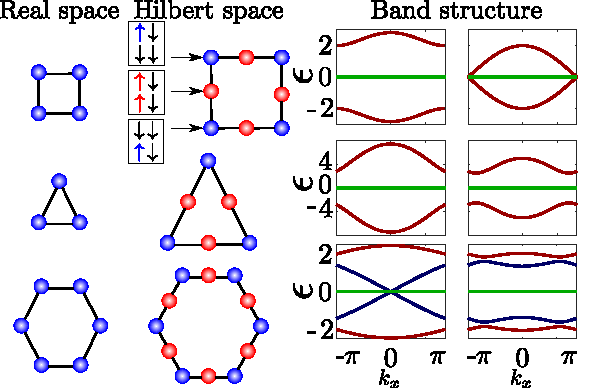
\includegraphics[width=\columnwidth]{lattices_real_hilbert_bands.pdf}
\caption{\textbf{Left column:} geometry of a square, a triangular, and a honeycomb lattice in real space. The blue dots depict the position of the Rydberg atoms and the lines the interaction between neighboring atoms. $R_0$ and $R_1$ represent nearest and next-nearest neighbor distances, respectively. \textbf{Middle column:} respective "synthetic lattices" in the Hilbert space under the facilitation conditions. The blue dots represent one-excitation states while the red spheres are pair states. \textbf{Right column:} Cut through the Brillouin zone for each lattice geometries at $k_y= 0$. Each lattice features (at least) a flat band. The momentum scales for the three lattices (from top to bottom) are $\eta=(R^{-1}_0,\tfrac{4}{3}R^{-1}_0,\tfrac{4}{3}R^{-1}_1).$}
\label{Fig:flat_band_lattices}
\end{figure}
%%
%%
%%
(i) in the original lattice structure, draw the links joining nearest neighbors; (ii) identify each site with the state having a single excitation on that site. This exhausts all ``one-excitation'' states in the subspace; (iii) each ``pair'' state can be straightforwardly associated to the link joining the two excited atoms; hence, place an additional site in the midpoint of each link and associate it with the corresponding ``pair'' state. The links in this new-found structure now effectively represent pair of states connected by the Hamiltonian, which can be therefore seen as a tight-binding model on a generalized synthetic lattice. In the case of a square lattice, the new structure (see Fig.~\ref{Fig:flat_band_lattices}) is called \emph{Lieb lattice} and is known to feature a flat band and two dispersive ones which meet with a linear dispersion at the edges of the first Brillouin zone. However, this construction is general and can be extended to any kind of regular \cite{footnote1} lattice. Most of these structures will support flat bands as well: It can be shown \cite{SM} that, calling $n_1$ ($n_2$) the number of one-excitation (pair) states in a unit cell, the number of flat bands $n_{\rm flat}$ must be $\geq \abs{n_1 - n_2}$. For the examples of Fig.~\ref{Fig:flat_band_lattices}, the square, triangular and honeycomb lattices have $(n_1,n_2,n_{\rm flat}) = (1,2,1)$, $(1,3,2)$ and $(2,3,1)$ respectively. These flat bands constitute extensively-degenerate eigenspaces of the Hamiltonian; as such, it is often possible to recombine the usual (plane-wave-like) Bloch solutions to form a set of localised eigenstates.

\emph{Disorder---} Disorder enters the picture through the uncertainty in the atomic positions. Even small displacements from the centre of the traps can significantly shift the atomic transitions off resonance from the laser frequency, thereby hindering the facilitation mechanism \cite{a_Marcuzzi_PRL_17}. In fact, the interaction potential seen by an atom at a distance $R = R_0 + \delta R$ from an excitation will be $V(R) = V(R_0 + \delta R) \equiv V(R_0) + \delta V$. 
%Note that, since $V(R) >0$, $\delta V > - V(R_0)$, i.e.~the energy shifts are only defined on a domain $[-V(R_0), +\infty)$. 
At small disorder ($\delta R \ll R_0$ and $\delta V \ll V(2R_0)$) the energy shifts can be approximated by $\delta V \approx -\alpha C_\alpha / R_0^{\alpha + 1} \delta R$. These random variables only affect pair states, creating a disordered potential landscape over the pair (red) sites in Fig.~\ref{Fig:flat_band_lattices}. The single-excitation (blue) sites' energy remains unvaried instead.

In order to characterize the disorder, we denote by $\omega$ the optical trapping frequency (assumed hereafter to be isotropic in space), by $m$ the atomic mass and by $T$ the temperature. The probability distribution of a trapped atom can then be approximately described as a Gaussian of width $\sigma$ around the trap centre. We require now that (I) $k_B T \gg \hbar \omega$: this implies that one can use the semiclassical estimate $\sigma \approx \sqrt{k_B T / m\omega^2}$ and moreover that the thermal de Broglie wavelength of the atom is much smaller than the distribution width. In other words, the atom can be approximately considered localized somewhere within the trap according to a classical probability distribution. (II) $\omega \Delta t \ll 1$, with $\Delta t$ the duration of an experiment: this ensures that the atoms will not appreciably move from their positions in this time frame and thus the disorder is quenched. (III) $\Omega \gg \omega$, or in other words the dynamics of the internal degrees of freedom is much faster than the one of the kinetic ones, so that within an experiment one can probe the action of the disordered Hamiltonian on the system while keeping the disorder quenched (i.e.~fixed). The properties of the probability distribution of energy shifts are discussed in \cite{SM}; here we just \changer{mention} that amplitudes of shifts over different pair sites are not independent, but correlated.

\emph{Disordered Lieb ladder---} In the remainder of our discussion, we shall focus on a ladder configuration, i.e.~a quasi-one-dimensional lattice formed by placing two linear chains parallel to each other at a lattice spacing distance $R_0$. For this example, the synthetic lattice (corresponding to the ``1D Lieb lattice'' case of Ref.~\cite{Leykam2017}) in the Hilbert space is sketched in Fig.~\ref{Fig:decoupling}(a). The unit cell consists of five sites with $n_1 = 2$ and $n_2 = 3$ and the band structure features one zero-energy flat and four dispersive bands [Fig.~\ref{Fig:decoupling}(d)].

\begin{figure}
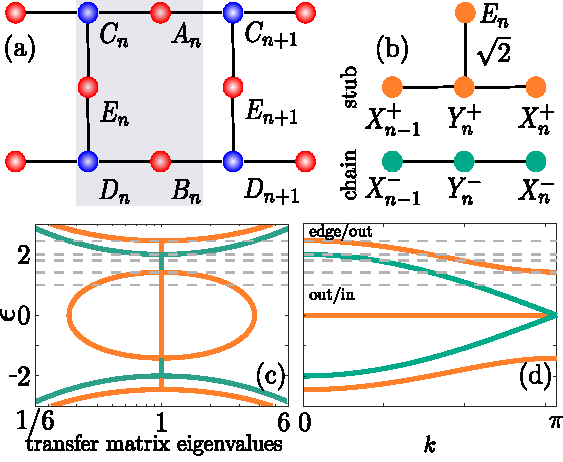
\includegraphics[width=\columnwidth]{decoupling.pdf}
\caption{Hilbert space structure and spectrum in the absence of disorder. \textbf{(a)} Lieb ladder. Blue spheres correspond to one-excitation states while red spheres represent pair states. We introduce a convenient notation for the five sites $A_n$, $B_n$, $C_n$, $D_n$, $E_n$ in the $n$-th unit cell (shaded grey). \textbf{(b)} A change of basis -- the so-called ``detangling'', introducing the new linear combinations $X_n^\pm = (A_n \pm B_n)/\sqrt{2}$ and $Y_n^\pm = (C_n \pm D_n)/\sqrt{2}$ \cite{a_Flach_EPL_14,Leykam2017} -- maps the Lieb ladder onto two decoupled chains. The $\sqrt{2}$ factor denotes that the hopping amplitude on the vertical link of each unit cell is amplified by that same amount. \textbf{(c)} Eigenvalues of the transfer matrix in log-linear scale. The dotted lines corresponds to the energies $\epsilon = \{0,1, \sqrt 2, 1.8, 2, \sqrt 6\}$ at which the scaling of the localization lengths is investigated in Fig.~\ref{Fig:2D_loc_length}. \textbf{(d)} Band structure of the Lieb ladder. The bands corresponding to the stub lattice are given in red and bands of the ordinary 1D chain are shown in green.}
\label{Fig:decoupling}
\end{figure}

This Lieb ladder constitutes one of the simplest examples where flat bands produce a non-trivial interplay with the on-site disorder \cite{Leykam2017}. In a Rydberg quantum simulator, however, the disorder only appears on pair states, i.e. all the blue sites of the synthetic lattice [Fig.~\ref{Fig:flat_band_lattices}(a)] are unaffected by it. To investigate the effect of this unusual disorder scenario we study in the following the scaling behaviour of the \emph{localization length} $\xi$ for small disorder strengths. \changer{This quantity encodes the localization properties of the energy eigenstates' wavefunctions, whose amplitude is typically peaked in a specific area of the lattice and decays exponentially as $\rme{-r/\xi}$ at large distances $r$.}

\changer{For a ladder like the one under study, two different values of $\xi$ can be extracted at any given energy, which we denote by $\xi_{1/2}$ and order according to $\xi_1 < \xi_2$. To elucidate the reason, one can perform an appropriate change of basis (``detangling transformation'' \cite{a_Flach_EPL_14,Leykam2017}) through which the Lieb ladder is mapped onto two uncoupled one-dimensional lattices [see Fig.~\ref{Fig:decoupling}(b)], a chain (in green, supporting the two innermost dispersive bands) and a stub lattice (in orange, supporting the flat and two outermost dispersive bands) \cite{SM}. At small disorder, one can thus associate either localization length to one of the two detangled chains.}
%
%
%
%Where possible, we connect our results to those presented in Ref.~\cite{Leykam2017}, where the same geometry is studied with independent disorder on all sites.
%
%Via an appropriate change of basis (``detangling transformation'' \cite{a_Flach_EPL_14,Leykam2017}) this Lieb ladder can be mapped onto two uncoupled one-dimensional lattices [see Fig.~\ref{Fig:decoupling}(b)], a chain (in green, supporting the two innermost dispersive bands) and a stub lattice (in orange, supporting the flat and two outermost dispersive bands) \cite{SM}. For every value of the energy, there are therefore two relevant localization lengths, denoted by $\xi_{1/2}$ with $\xi_1 < \xi_2$. These are associated with the localization properties of either of the detangled chains of Fig.~\ref{Fig:decoupling}(b), i.e. the wave functions are peaked and mostly concentrated in a specific area of the chainw and decay as $\rme{-r/\xi_{1/2}}$ with the distance $r$.

The values $\xi_{1/2}$ are found numerically via a transfer matrix formalism and are displayed in Fig.~\ref{Fig:2D_loc_length}(a) as a function of $s \equiv \sigma / R_0$ and the energy $\epsilon$.
\begin{figure}
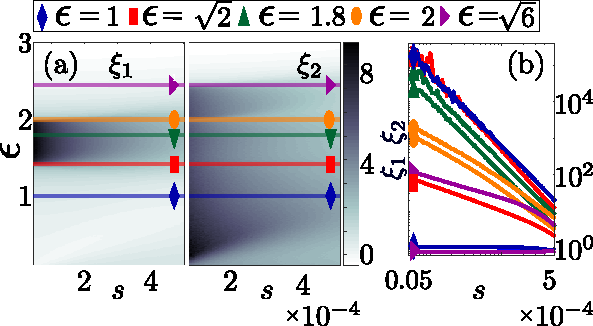
\includegraphics[width=\columnwidth]{loc_length_dipole_BW_new.pdf}
\caption{\textbf{(a)} Localization lengths $\xi_1,\,\xi_2$ as a function of the energy $\epsilon$ and the disorder strength $s = \sigma / R_0$.
\textbf{(b)} Localization lengths along each of the solid lines displayed in panel (a) in log-log scale. For small disorder all lines are approximately linear which allows to assign approximate power law exponents $\nu$ characterizing the small-disorder behavior $\xi_i \sim s^\nu$: grouping them by energy $\epsilon$, they read $\nu\left(\epsilon = 1\right) \approx$ \{0.1, 2.0\}, $\nu\left(\epsilon = \sqrt{2}\right)\approx$ \{0.8, 2.2\}, $\nu\left(\epsilon = 1.8\right)\approx$ \{2.0, 2.0\}, $\nu\left(\epsilon = 2\right)\approx$ \{1.4, 1.4\}, $\nu\left(\epsilon = \sqrt{6}\right)\approx$ \{0.0, 0.8\}. For these computations we chose a dipole-dipole interaction ($\alpha = 3$) with an interaction strength of $V_0 = 300\Omega$.}
 \label{Fig:2D_loc_length}
\end{figure}
In Fig.~\ref{Fig:2D_loc_length}(b) we display log-log plots of the correlation lengths at selected energies as functions of $s$, which illustrate algebraic scaling $\xi_i \sim s^\nu$, for sufficiently small $s$. \changer{Where possible, we connect our findings to those presented in Ref.~\cite{Leykam2017}, where the same geometry is studied with independent disorder on all sites. The usual scaling for Anderson localization corresponds to $\nu = 0$ at energies outside a band (``out''), $\nu = 2/3$ at a band edge (``edge'') and $\nu = 2$ inside a band (``in''). The energies selected in Fig.~\ref{Fig:decoupling} correspond to $\epsilon =1$ (out/in), $\sqrt{2}$ (edge/in), $1.8$ (in/in), $2$ \changer{(in/edge)} and $\sqrt{6}$ \changer{(edge/out)}. Here the entries in the brackets refer to the two band structures depicted in Fig.~\ref{Fig:decoupling}(c,d): (red/green).}

In Ref.~\cite{Leykam2017} an ``anomalous'' scaling $\nu = 4/3$ was found in at $\epsilon = \sqrt{2}$ and $2$. This was attributed to the fact that disorder, in the detangled picture, is not merely on-site but couples the two chains; this in turn may produce resonances between states in the middle of a band and states at the edge of the other one when the latter displays vanishing group velocity. Comparing these values with the ones obtained for our situation, we observe reasonable agreement at $\epsilon = 1$ and $\epsilon = 1.8$, for the anomalous scaling at $\epsilon = 2$ and for the ``out'' scaling at $\epsilon = \sqrt{6}$. The anomalous scaling at $\epsilon = \sqrt{2}$ seems instead to be ``cured'' as we retrieve a result compatible with the usual Anderson one ($\nu  \approx 2$). This is likely to be due \mm{supplemental or not?} to the alternating structure of the disorder in the synthetic lattice, which in the detangled picture results in the absence of random couplings between $Y_n^{\pm}$ sites [see Fig. \ref{Fig:decoupling}(b)], which were present instead in Ref. \cite{Leykam2017}.

For energies located at the ``edge'' we observe \changer{two instances of $\nu$ of approximately $0.8$ at $\epsilon = \sqrt{2}$ and $\sqrt{6}$;l these values are still sufficiently close to the expected $2/3$, in particular considering that, due to numerical imitations, we were unable to push our numerical exploration to smaller values of $s$. However, at $\epsilon = 2$ we find an exponent of approximately $1.4$. This is not close to the Anderson value $2/3$ but is similar to the anomalous exponent $4/3$ discussed above. An explanation for this behavior is currently lacking and requires further investigations.}


%
% discrepancies in comparison to Ref. \cite{Leykam2017}: the exponents at $\epsilon = \sqrt{2}$ and $\sqrt{6}$ are $0.8$ \changer{but may still be regarded as close enough to the value $2/3$ identified in} \cite{Leykam2017}. However, at $\epsilon = 2$ we find an exponent of approximately $1.4$. This is not close to the Anderson value $2/3$ but is similar to the anomalous exponent $4/3$ discussed above. An explanation for this behavior is currently lacking and will be subject to further studies.

\emph{Localized state dynamics---}
\begin{figure}
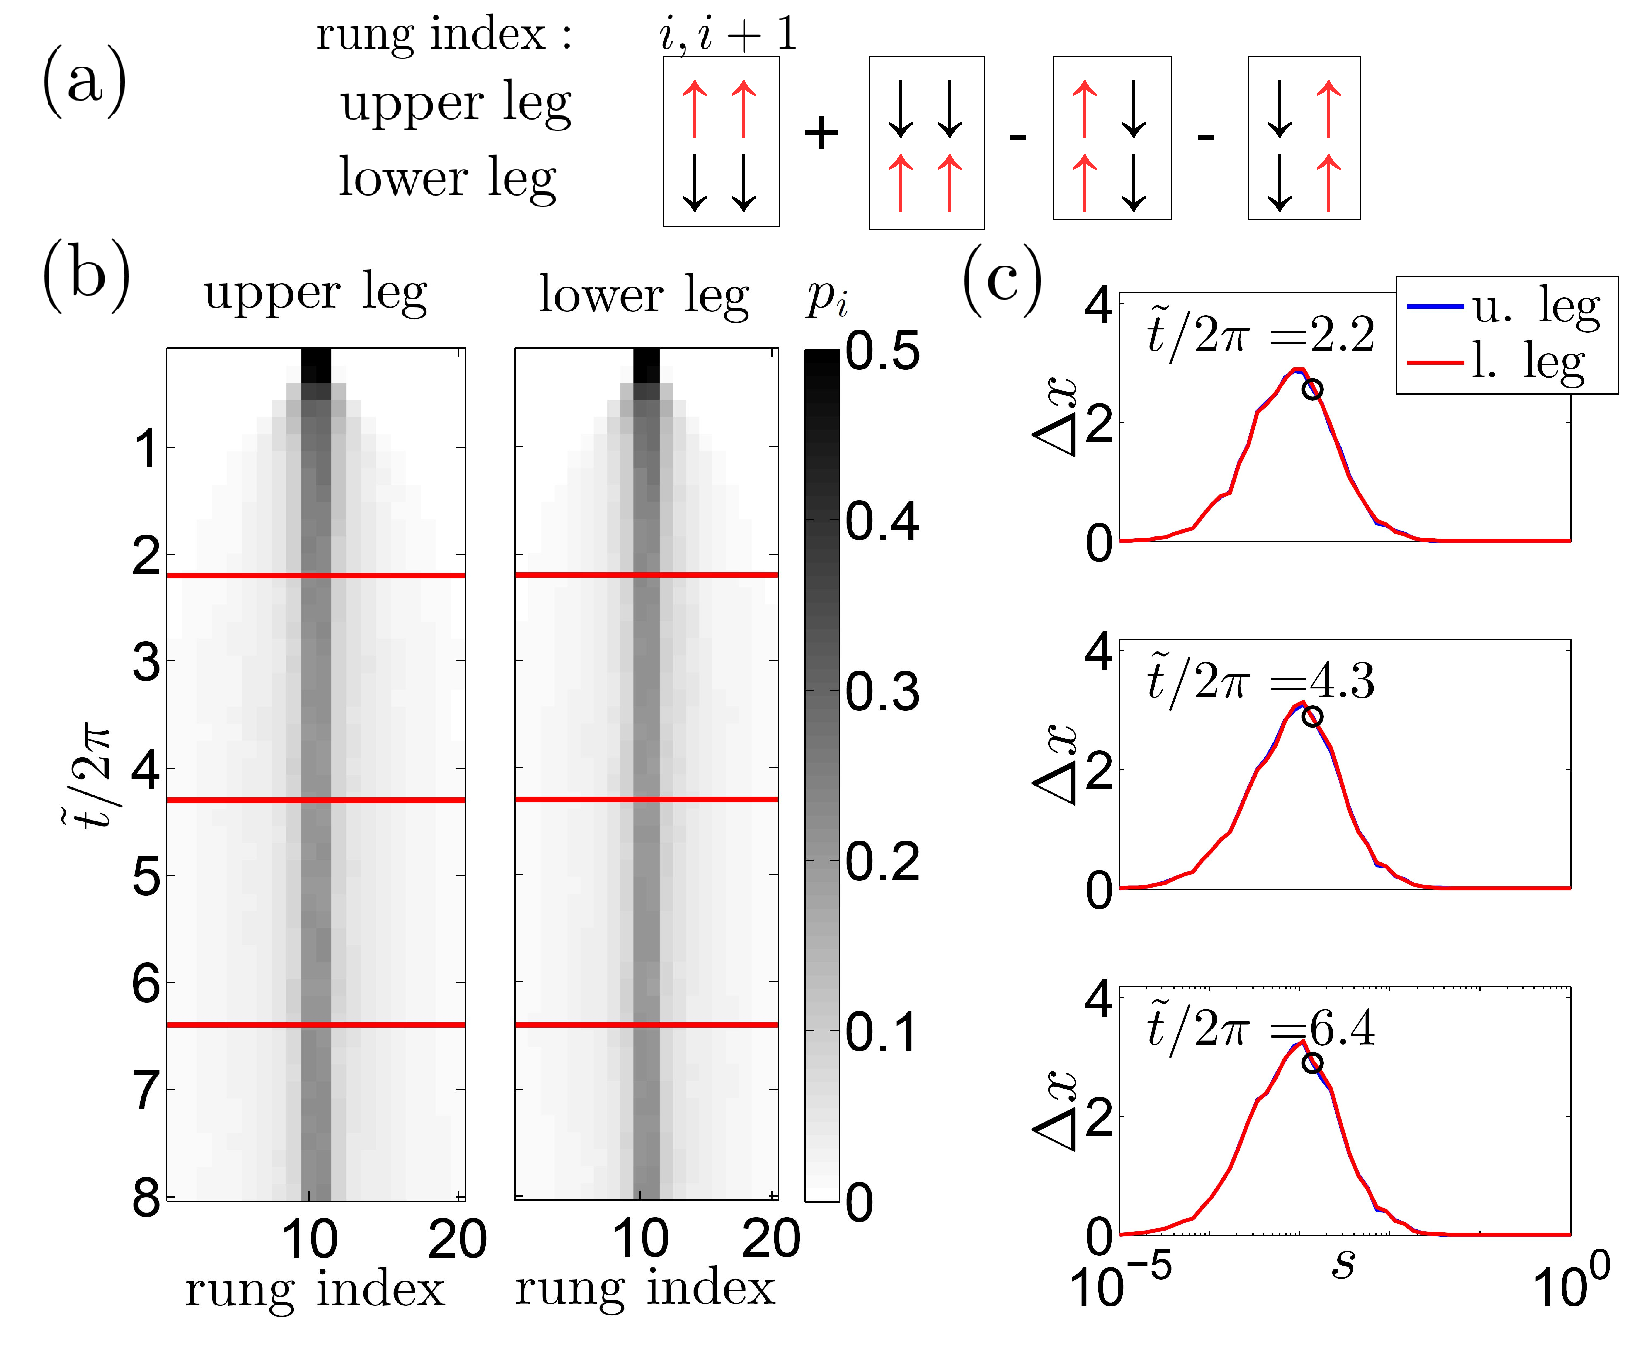
\includegraphics[width=\columnwidth]{time_evolution_CLS_PaperSupport_v4.pdf}
\caption{\textbf{(a)} Schematic representation of the spin configuration corresponding to the initial state $\ket{\psi_{\rm loc}}$ localized at rungs $i,i+1$ of the ladder. \textbf{(b)} The probability of excitations $p_i$ given by the time evolution of the localized state with an initial support in the middle (rungs $10$ and $11$) of the ladder of length $20$ for $s=0.0014$. The left (right) pane shows the time evolution in the upper (lower) leg of the ladder. The horizontal red lines denote three different times for which the respective value of $\Delta x$ is shown as a black circle in (c). \textbf{(c)} Standard deviation of the excitation positions $\Delta x$ vs. the disorder strength $s$ for three different times. Blue (red) solid lines, which are virtually indistinguishable correspond to upper (lower) leg of the ladder respectively. Results obtained for $100$ disorder realizations and $V_0=200\Omega$.}
\label{Fig:time evolution}
\end{figure}
Experimentally measuring the localization lengths studied above is challenging due to the required large systems size and small disorder amplitudes. However, one can probe the influence of disorder by initializing the system in a specific state and tracking the subsequent dynamics by measuring the on-site excitation probabilities \cite{Schauss_2015,Labuhn_2015,Bernien2017}. A particularly interesting choice for an initial state is localized and an eigenstate of the flat band. Such state is no propagating in the absence of disorder. We show in \cite{SM} that it takes the form $\ket{\psi_{\rm loc}} = 1/\sqrt{4} \left( \ket{A_i} + \ket{B_i} - \ket{E_i} - \ket{E_{i+1}} \right)$, being entirely localized at rungs $i,i+1$ of the ladder [see Fig. \ref{Fig:time evolution}(a)]. States of this form can be prepared experimentally via single site addressing (for the protocol see \cite{SM}).

The time evolution of the excitation density is shown in Fig. \ref{Fig:time evolution}(b). The effect of the disorder becomes apparent in the width $\Delta x$ \changer{(see \cite{SM} for the formal definition)} of the density packet which quickly reaches a stationary state. It is interesting to observe that, as shown in Fig.~\ref{Fig:time evolution}(c), the stationary value of $\Delta x$ shows a non-monotonic behavior as a function of $s$. This can be understood as follows: at very small (but finite) $s$ the initial state (energy $\epsilon \approx 0$) is almost an flat band eigenstate and it therefore only minimally spreads. As $s$ is increased, this picture breaks down and the state more and more strongly connects to other ones, allowing transport to larger distances. At the same time, however, the localization lengths at $\epsilon = 0$ decrease. Hence, an interplay ensues: the spreading $\Delta x$ of the state increases with $s$ as long as the localization length remains larger ($\Delta x \ll \xi_i$). Once the decrease in the localization scale catches up with the increase of $\Delta x$, the behavior is dominated by localization and, as expected, decreases with increasing disorder strength.

\emph{Conclusions and Outlook---} We have shown that Rydberg quantum simulators allow to explore localization phenomena in synthetic lattices with flat bands and unconventional types of disorder (correlated, alternating). The current study focuses on the Lieb ladder and on a particular excitation sector. Higher-dimensional lattices hosting more excitations are straight-forwardly realizable in experiment. It is thus a future theoretical challenge to shed light on these intricate and unexplored scenarios.

\emph{Acknowledgments---} The research  leading  to  these  results  has  received  funding  from the European Research Council under the European Union’s Seventh Framework Programme (FP/2007-2013)/ERC Grant Agreement No.
335266 (ESCQUMA), the EPSRC Grant No. EP/M014266/1, and the H2020-FETPROACT-2014 Grant No. 640378 (RYSQ). I.L. gratefully acknowledges funding through the Royal Society Wolfson Research Merit Award.

\bibliographystyle{apsrev4-1}

\bibliography{bibliography}


\end{document} 